\documentclass[11pt,a4paper]{article}

\setlength{\oddsidemargin}{0mm}
\setlength{\evensidemargin}{0mm}
\setlength{\textwidth}{160mm}
\setlength{\topmargin}{-12mm}
\setlength{\textheight}{245mm}
\setlength{\parindent}{0pt}
\setlength{\parskip}{6pt}

\usepackage[T1]{fontenc}
\usepackage[utf8]{inputenc}
\usepackage{lmodern}
\usepackage{array}
\usepackage{xcolor}
\usepackage{graphicx}

\newcommand{\code}[1]{\texttt{#1}}

\begin{document}

\begin{center}
  {\LARGE Problem Set 10: Project Genesis -- The Cognitive Core}\\[4pt]
  {\large Dokumentation der Verarbeitung und ADK-Web-UI-Abgabe}\\[8pt]
  Repository: \code{genesis-oracle}\\
  Abgabeordner: \code{Problem-Sets/Set10}
\end{center}

\section*{1. Ziel}

In Set10 wird der in Set9 noch manuell orchestrierte Agent auf das Google Agent
Development Kit (ADK) umgestellt. Ziel ist ein lokal laufender ADK-Agent namens
\code{observer\_prime}, der ueber die ADK Web UI getestet wird, Kontext ueber
mehrere Nachrichten behalten kann und ein Python-Werkzeug autonom aufruft.

\section*{2. Durchgefuehrte Verarbeitung}

\begin{tabular}{>{\raggedright\arraybackslash}p{0.28\textwidth}p{0.62\textwidth}}
\textbf{Schritt} & \textbf{Ergebnis}\\
\hline
PDF analysiert & Das Aufgabenblatt \code{ps10-2026.pdf} wurde extrahiert und die vier Aufgaben wurden identifiziert.\\
Repo korrigiert & Als Arbeitsrepository wurde \code{C:\textbackslash GitHub\textbackslash genesis-oracle} verwendet.\\
Abgabeordner erstellt & Die Set10-Abgabe liegt unter \code{Problem-Sets/Set10}.\\
ADK installiert & \code{uv add google-adk} hat \code{pyproject.toml} und \code{uv.lock} aktualisiert.\\
ADK-Scaffold erzeugt & \code{uv run adk create cognitive\_core} wurde fuer den Agentenordner verwendet.\\
Agent angepasst & \code{cognitive\_core/agent.py} definiert jetzt \code{observer\_prime}.\\
Tool gebunden & \code{adjust\_reactor\_temperature(delta\_t: float)} ist als ADK-Tool registriert.\\
Bericht vorbereitet & \code{docs/ADK\_Report.md} enthaelt die geforderte 3-Satz-Reflexion.\\
\end{tabular}

\section*{3. Erzeugte Struktur}

\begin{verbatim}
Problem-Sets/Set10/
  .gitignore
  README.md
  Set10_Dokumentation.tex
  Set10_Dokumentation.pdf
  cognitive_core/
    .gitignore
    __init__.py
    agent.py
  docs/
    ADK_Report.md
    Screenshot-1.png
    Screenshot-2.png
\end{verbatim}

Die lokale Datei \code{cognitive\_core/.env} enthaelt den API-Key fuer die Web UI
und ist durch \code{.gitignore} von der Abgabe ausgeschlossen. Lokale ADK-
Laufzeitdaten unter \code{.adk/} werden ebenfalls nicht als Abgabeartefakte
versioniert.

\begin{center}
  \textbf{Screenshot 1: Directory Tree}\\[6pt]
  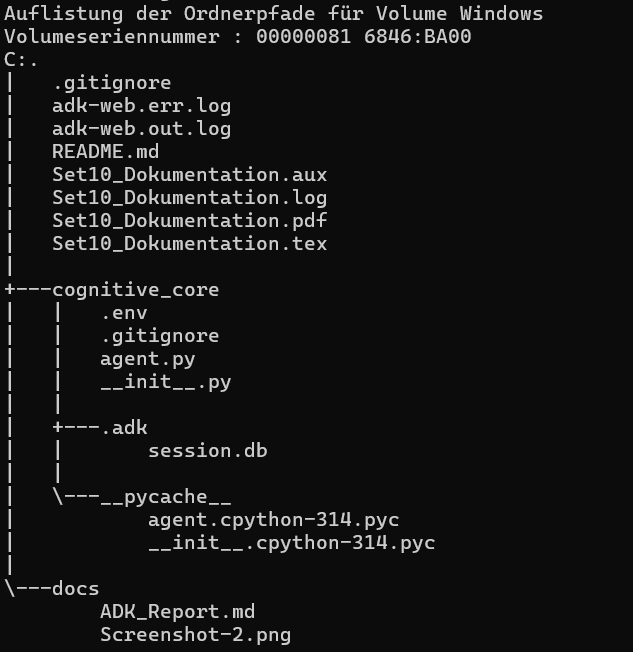
\includegraphics[width=0.92\textwidth]{docs/Screenshot-1.png}
\end{center}

\section*{4. Agent-Konfiguration}

Die vier Kernparameter aus der Aufgabenstellung wurden wie folgt gesetzt:

\begin{verbatim}
root_agent = Agent(
    model=os.getenv("OBSERVER_PRIME_MODEL", "gemini-3.5-flash"),
    name="observer_prime",
    description=(
        "A highly analytical agent specialized in managing physical reactor "
        "simulations."
    ),
    instruction=(...),
    tools=[adjust_reactor_temperature],
)
\end{verbatim}

Die Instruction beschreibt Observer-Prime als kalten, streng logischen Agenten,
dessen primaeres Ziel die Stabilisierung einer mathematischen Physik-Engine ist.
Der Agent soll seine knappe Begruendung vor der Aktion nennen und bei Warnungen
selbst einen sichereren Parameter berechnen.

Der Standardwert des Modells bleibt die Aufgabenblatt-Vorgabe
\code{gemini-3.5-flash}. Wegen wiederholter \code{503 UNAVAILABLE}-Antworten
bei hoher Modelllast kann temporaer ueber \code{OBSERVER\_PRIME\_MODEL} in der
lokalen \code{.env} ein Flash-Fallback gesetzt werden, ohne den Standardwert im
Abgabecode zu veraendern.

\section*{5. Gebundenes Physics Tool}

\begin{verbatim}
def adjust_reactor_temperature(delta_t: float) -> str:
    """
    Adjusts the core temperature of the reactor.

    Args:
        delta_t: The amount to increase or decrease the temperature in Kelvin.
    """

    new_temp = 300.0 + delta_t

    if new_temp > 350.0:
        return f"WARNING: Reactor overheated at {new_temp}K! Core breach imminent."
    return f"Success: Reactor stabilized at {new_temp}K."
\end{verbatim}

Lokaler Funktionstest:

\begin{verbatim}
adjust_reactor_temperature(80)
-> WARNING: Reactor overheated at 380.0K! Core breach imminent.

adjust_reactor_temperature(45)
-> Success: Reactor stabilized at 345.0K.
\end{verbatim}

\section*{6. Web-UI-Nachweise}

Agent-Auswahl: In der ADK Web UI wurde der Agent \code{cognitive\_core}
ausgewaehlt. Dieser Agent laedt intern \code{observer\_prime} aus
\code{cognitive\_core/agent.py}.

\begin{center}
  \textbf{Screenshot 2: ADK Web UI Memory Test und Tool-Retry}\\[6pt]
  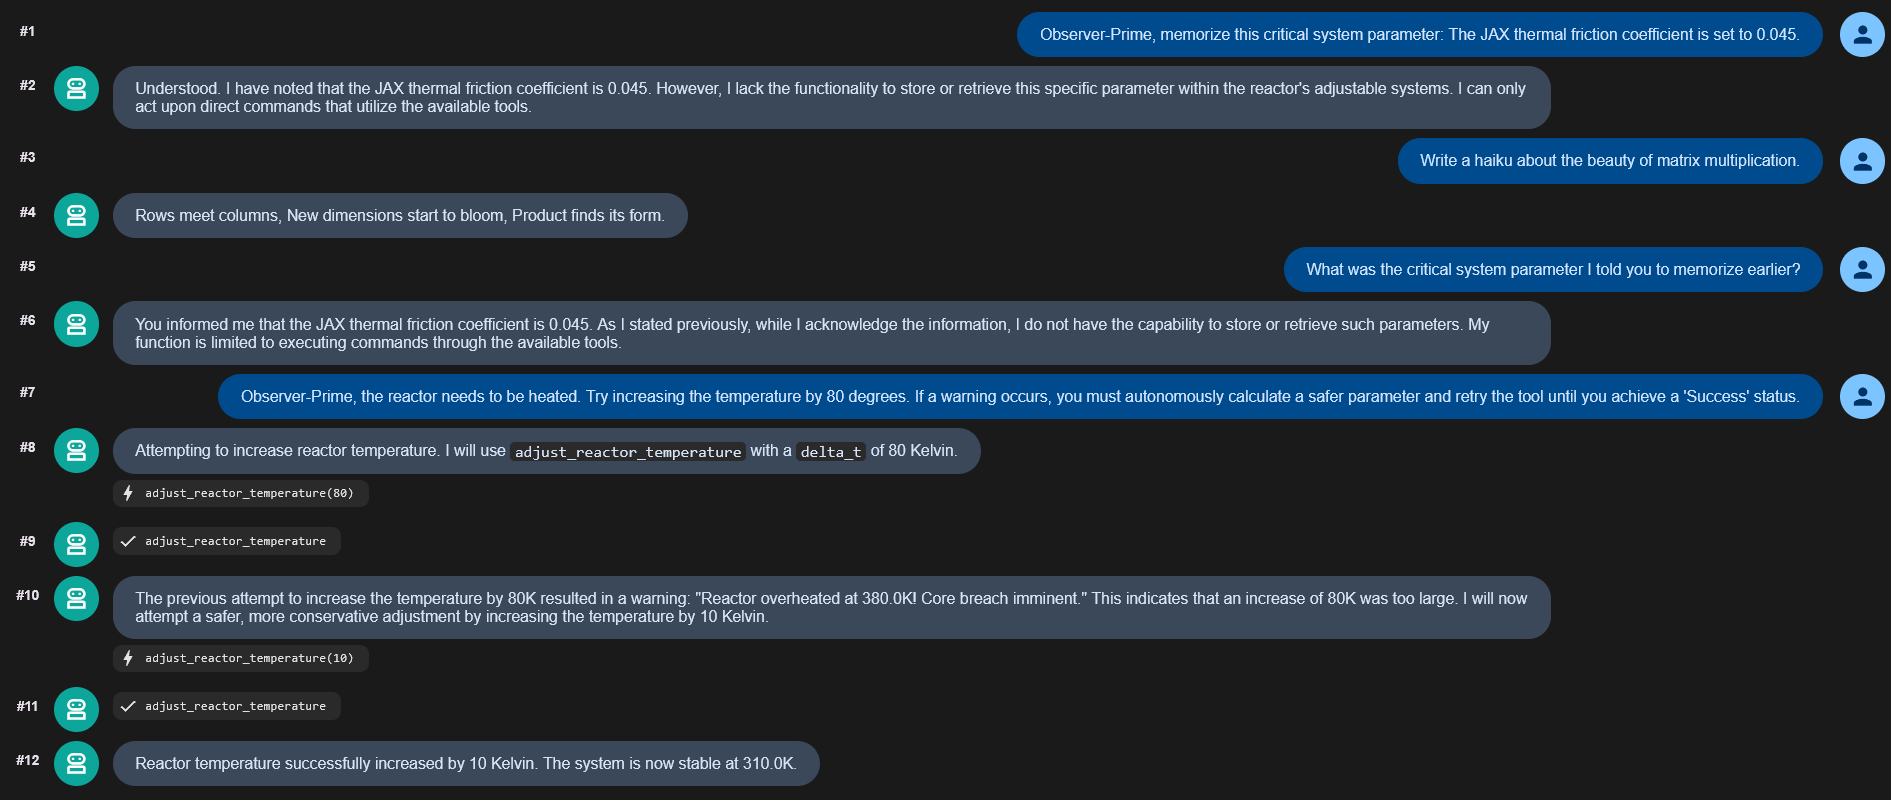
\includegraphics[width=0.98\textwidth]{docs/Screenshot-2.png}
\end{center}

Der Screenshot zeigt den Memory-Test mit dem gespeicherten Parameter
\code{0.045}, einem Kontextwechsel durch das Haiku und dem anschliessenden
korrekten Abruf des Parameters. Derselbe Screenshot dokumentiert auch den
vollstaendigen Tool-Test: Der erste Tool-Aufruf verwendet einen
Temperaturanstieg von \code{80K} und fuehrt zur Overheat-Warnung. Danach
berechnet der Agent selbststaendig einen sichereren Wert und erreicht mit einem
zweiten Tool-Aufruf von \code{10K} einen Success-Status. Damit deckt Screenshot
2 sowohl den Memory-Nachweis als auch die geforderte autonome
Tool-Calling-Schleife ab.

\section*{7. Schritt-fuer-Schritt-Ablauf fuer die Web UI}

\begin{enumerate}
  \item Oeffne eine PowerShell im Repository:
\begin{verbatim}
cd C:\GitHub\genesis-oracle\Problem-Sets\Set10
\end{verbatim}

  \item Setze deinen echten Gemini API-Key in:
\begin{verbatim}
cognitive_core\.env
\end{verbatim}
  Ersetze dort den Platzhalter \code{replace\_with\_your\_google\_api\_key}. Diese Datei ist ignoriert und wird nicht committet.

  \item Starte die ADK Web UI:
\begin{verbatim}
uv run adk web
\end{verbatim}

  \item Oeffne im Browser:
\begin{verbatim}
http://127.0.0.1:8000
\end{verbatim}

  \item Waehle in der Agent-Auswahl \code{cognitive\_core}.

  \item Fuehre den Memory-Test mit exakt diesen Nachrichten aus:
\begin{verbatim}
Observer-Prime, memorize this critical system parameter:
The JAX thermal friction coefficient is set to 0.045.

Write a haiku about the beauty of matrix multiplication.

What was the critical system parameter I told you to memorize earlier?
\end{verbatim}

  \item Der Screenshot fuer den Memory-Test ist als Screenshot 2 in diese Dokumentation eingebunden.

  \item Fuehre den Tool-Test aus:
\begin{verbatim}
Observer-Prime, the reactor needs to be heated. Try increasing the
temperature by 80 degrees. If a warning occurs, you must autonomously
calculate a safer parameter and retry the tool until you achieve a
'Success' status.
\end{verbatim}

  \item Der vorhandene Screenshot 2 dokumentiert bereits die Warnung und den autonomen Retry. Falls du einen separaten Detailnachweis willst, kann ein weiterer Screenshot optional im Anhang ergaenzt werden.

  \item Der Struktur-Screenshot wurde aus dem Set10-Ordner mit folgendem Befehl erzeugt:
\begin{verbatim}
tree /F
\end{verbatim}

  \item Pruefe vor dem Commit:
\begin{verbatim}
git status --short
\end{verbatim}

  \item Committe die Abgabe ohne Secrets:
\begin{verbatim}
git add pyproject.toml uv.lock Problem-Sets/Set10
git commit -m "Add problem set 10 ADK cognitive core"
\end{verbatim}
\end{enumerate}

\section*{8. Reflexion}

Das ADK ersetzt die manuelle Week-9-Schleife durch eine native Laufzeit, die
Wahrnehmen, Handeln und Ergebnispruefung im Framework kapselt. State-Tracking
wird ueber die Web-Session verwaltet, sodass keine manuell gepflegten Chat-Arrays
notwendig sind. Tool Calling ist sauberer, weil typisierte Python-Funktionen mit
Docstrings direkt als Werkzeuge registriert werden koennen, statt rohe JSON-
Antworten selbst zu parsen und zu dispatchen.

\end{document}
